\subsection{INVERSE LIMITS OF ALGEBRAIC STRUCTURES}

Let \((\mathbf{X}_{\alpha}, f_{\alpha\beta})\) be an inverse system of sets, and suppose that each \(X_{\alpha}\) is endowed with an internal law of composition, everywhere defined, and written multiplicatively. Suppose also that the \(f_{\alpha\beta}\) are homomorphisms with respect to these internal laws. Since

\[
f _ {\alpha \beta} (x _ {\beta}. y _ {\beta}) = f _ {\alpha \beta} (x _ {\beta}). f _ {\alpha \beta} (y _ {\beta})
\]

whenever \(\alpha \leqslant \beta\) and \(x_{\beta}\) and \(y_{\beta}\) belong to \(\mathbf{X}_{\beta}\) , it is clear that \(\mathbf{X} = \varprojlim \mathbf{X}_{\alpha}\) is a stable subset of the product \(\prod_{\alpha} \mathbf{X}_{\alpha}\) , with respect to the internal law \((x_{\alpha}) \cdot (y_{\alpha}) = (x_{\alpha} \cdot y_{\alpha})\) . Let \((\Lambda_{\alpha}, \varphi_{\alpha\beta})\) be another inverse system of sets, indexed by I, and suppose that each \(\mathbf{X}_{\alpha}\) carries an external law of composition, everywhere defined, written multiplicatively and having \(\Lambda_{\alpha}\) as a set of operators, such that whenever \(\alpha \leqslant \beta\) we have

\[
f _ {\alpha \beta} (\lambda_ {\beta}. x _ {\beta}) = \varphi_ {\alpha \beta} (\lambda_ {\beta}). f _ {\alpha \beta} (x _ {\beta})
\]

for \(\lambda_{\beta} \in \Lambda_{\beta}\) and \(x_{\beta} \in X_{\beta}\) . Then we can define an external law on \(\prod_{\alpha} X_{\alpha}\) , having \(\prod_{\alpha} \Lambda_{\alpha}\) as a set of operators, by defining \((\lambda_{\alpha}) \cdot (x_{\alpha}) = (\lambda_{\alpha} \cdot x_{\alpha})\) ; restricting the set of operators to \(\Lambda = \varprojlim \Lambda_{\alpha}\) , we have an external law on \(\prod_{\alpha} X_{\alpha}\) with respect to which \(X\) is again a stable subset. The internal

(resp. external) law thus defined on X is said to be the inverse limit of the internal (resp. external) laws of the \(X_{\alpha}\) . In the case of external laws, it may happen that all the \(\Lambda_{\alpha}\) are identical with the same set \(\Lambda_{0}\) and that all the \(\varphi_{\alpha \beta}\) are identity mappings; then, since I is a directed set, \(\Lambda\) can be identified with \(\Lambda_0\) .

It is immediately verified that the usual properties of associativity, commutativity, existence of an identity element for an internal law (provided that the \(f_{\alpha\beta}\) map identity element to identity element), distributivity of an external law with respect to an internal law, etc., are preserved under passage to the inverse limit.

Let \(\Sigma\) be a species of algebraic structure and let \(\Sigma_0\) be the impoverished structure corresponding to \(\Sigma\) . Whenever we speak of an inverse system of sets \((\mathbf{X}_{\alpha}, f_{\alpha\beta})\) endowed with structures of species \(\Sigma\) , we shall always suppose that the \(f_{\alpha\beta}\) are homomorphisms for these structures. If we endow \(\mathbf{X} = \varprojlim \mathbf{X}_{\alpha}\) with the internal and external laws which are the respective inverse limits of the internal and external laws of the \(\mathbf{X}_{\alpha}\) , then \(\mathbf{X}\) carries an algebraic structure of species \(\Sigma_0\) . Naturally it remains to be seen in each particular case whether or not this structure is of species \(\Sigma\) .

For example, if \((\mathbf{G}_{\alpha}, f_{\alpha\beta})\) is an inverse system of groups (resp. rings), then \(\varprojlim G_{\alpha}\) is a subgroup (resp. subring) of \(\prod_{\alpha} G_{\alpha}\) , and is called the inverse limit of the system \((\mathbf{G}_{\alpha}, f_{\alpha\beta})\) of groups (resp. rings).

Let \((\mathbf{X}_{\alpha}, g_{\alpha \beta})\) be an inverse system of sets and let \((\mathbf{G}_{\alpha}, f_{\alpha \beta})\) be an inverse system of groups; suppose that each \(\mathbf{X}_{\alpha}\) has \(\mathbf{G}_{\alpha}\) as a group of operators and that whenever \(\alpha \leqslant \beta\) we have

\[
g _ {\alpha \beta} (s _ {\beta}. x _ {\beta}) = f _ {\alpha \beta} (s _ {\beta}). g _ {\alpha \beta} (x _ {\beta})\tag{1}
\]

for \(x_{\beta} \in X_{\beta}\) and \(s_{\beta} \in G_{\beta}\) . Then \(X = \varprojlim X_{\alpha}\) has \(G = \varprojlim G_{\alpha}\) as group of operators. It follows from (1) that, if \(\alpha \leqslant \beta\) , the mappings \(f_{\alpha \beta}\) and \(g_{\alpha \beta}\) are compatible (§ 2, no. 4) and hence define a mapping \(\varphi_{\alpha \beta}: X_{\beta}/G_{\beta} \to X_{\alpha}/G_{\alpha}\) of the quotient sets, such that \((X_{\alpha}/G_{\alpha}, \varphi_{\alpha \beta})\) is an inverse system. Moreover, if \(f_{\alpha}: G \to G_{\alpha}\) and \(g_{\alpha}: X \to X_{\alpha}\) are the canonical mappings, then \(f_{\alpha}\) and \(g_{\alpha}\) are compatible and consequently define a mapping \(h_{\alpha}: X/G \to X_{\alpha}/G_{\alpha}\) of the quotient sets; it is clear that the \(h_{\alpha}\) form an inverse system of mappings, whose inverse limit is therefore a mapping \(h: X/G \to \varprojlim X_{\alpha}/G_{\alpha}\) , which is not necessarily either injective or surjective (Exercise 1).

Again, let \((\mathbf{A}_{\alpha}, \varphi_{\alpha\beta})\) be an inverse system of rings and let \((\mathbf{M}_{\alpha}, f_{\alpha\beta})\) be an inverse system of commutative groups; and suppose that each \(M_{\alpha}\) carries a left \(A_{\alpha}\) -module structure in such a way that whenever \(\alpha \leqslant \beta\) we have

\[
f _ {\alpha \beta} (\lambda_ {\beta}. x _ {\beta}) = \varphi_ {\alpha \beta} (\lambda_ {\beta}). f _ {\alpha \beta} (x _ {\beta})\tag{2}
\]

for \(x_{\beta} \in M_{\beta}\) and \(\lambda_{\beta} \in A_{\beta}\) ; then \(\varprojlim M_{\alpha}\) has a structure of a left module over \(\varprojlim A_{\alpha}\) . If we suppose in addition that, for each \(\alpha\) , \(A_{\alpha}\) is commutative and that each \(M_{\alpha}\) has an \(A_{\alpha}\) -algebra structure, and finally that \((\mathbf{M}_{\alpha}, f_{\alpha\beta})\) is an inverse system of rings, then \(\varprojlim M_{\alpha}\) has a structure of an algebra over \(\varprojlim A_{\alpha}\) .

Let \((\mathbf{G}_{\alpha}, f_{\alpha \beta})\) be an inverse system of groups, and for each \(\alpha\) let \(\mathbf{H}_{\alpha}\) be a subgroup of \(\mathbf{G}_{\alpha}\) . If \(f_{\alpha \beta}(\mathbf{H}_{\beta}) \subset \mathbf{H}_{\alpha}\) whenever \(\alpha \leqslant \beta\) , then the inverse system of subsets \(\mathbf{H}_{\alpha}\) of \(\mathbf{G}_{\alpha}\) is an inverse system of groups with respect to the restrictions of the \(f_{\alpha \beta}\) , and \(\mathbf{H} = \varprojlim \mathbf{H}_{\alpha}\) is a subgroup of \(\mathbf{G} = \varprojlim \mathbf{G}_{\alpha}\) . If each \(\mathbf{H}_{\alpha}\) is a normal subgroup of \(\mathbf{G}_{\alpha}\) , then \(\mathbf{H}\) is a normal subgroup of \(\mathbf{G}\) . If \((\mathbf{G}_{\alpha}', f_{\alpha \beta}')\) is another inverse system of groups and, for each \(\alpha, u_{\alpha}: \mathbf{G}_{\alpha} \to \mathbf{G}_{\alpha}'\) is a homomorphism such that the \(u_{\alpha}\) form an inverse system of mappings, then, if \(\mathbf{H}_{\alpha}\) is the kernel of \(u_{\alpha}\) , we have \(f_{\alpha \beta}(\mathbf{H}_{\beta}) \subset \mathbf{H}_{\alpha}\) whenever \(\alpha \leqslant \beta\) ; \(u = \varprojlim u_{\alpha}\) is a homomorphism of \(\mathbf{G}\) into \(\mathbf{G}' = \varprojlim \mathbf{G}_{\alpha}'\) , and \(\mathbf{H} = \varprojlim \mathbf{H}_{\alpha}\) is the kernel of \(u\) . If we put \(\mathbf{K}_{\alpha} = u_{\alpha}(\mathbf{G}_{\alpha})\) , then we have \(f_{\alpha\beta}'(\mathbf{K}_{\beta}) \subset \mathbf{K}_{\alpha}\) whenever \(\alpha \leqslant \beta\) , so that the \(\mathbf{K}_{\alpha}\) form an inverse system of subgroups of the \(\mathbf{G}_{\alpha}'\) ; but \(\mathbf{K} = \varprojlim \mathbf{K}_{\alpha}\) is not necessarily the image of \(\mathbf{G}\) under \(u\) {[}Exercise 1 c){]}.

\pandocbounded{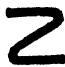
\includegraphics[keepaspectratio]{images/part002_764ec905.jpg}}

We obtain analogous results by replacing ``group'' by ``ring'', ``subgroup'' by ``ideal'' (left or right); we leave to the reader the task of stating the analogous results for modules and algebras.

